%
\documentclass{article} % For LaTeX2e
\usepackage{iclr2021_conference,times}

% Optional math commands from https://github.com/goodfeli/dlbook_notation.
%%%%% NEW MATH DEFINITIONS %%%%%

\usepackage{amsmath,amsfonts,bm}

% Mark sections of captions for referring to divisions of figures
\newcommand{\figleft}{{\em (Left)}}
\newcommand{\figcenter}{{\em (Center)}}
\newcommand{\figright}{{\em (Right)}}
\newcommand{\figtop}{{\em (Top)}}
\newcommand{\figbottom}{{\em (Bottom)}}
\newcommand{\captiona}{{\em (a)}}
\newcommand{\captionb}{{\em (b)}}
\newcommand{\captionc}{{\em (c)}}
\newcommand{\captiond}{{\em (d)}}

% Highlight a newly defined term
\newcommand{\newterm}[1]{{\bf #1}}


% Figure reference, lower-case.
\def\figref#1{figure~\ref{#1}}
% Figure reference, capital. For start of sentence
\def\Figref#1{Figure~\ref{#1}}
\def\twofigref#1#2{figures \ref{#1} and \ref{#2}}
\def\quadfigref#1#2#3#4{figures \ref{#1}, \ref{#2}, \ref{#3} and \ref{#4}}
% Section reference, lower-case.
\def\secref#1{section~\ref{#1}}
% Section reference, capital.
\def\Secref#1{Section~\ref{#1}}
% Reference to two sections.
\def\twosecrefs#1#2{sections \ref{#1} and \ref{#2}}
% Reference to three sections.
\def\secrefs#1#2#3{sections \ref{#1}, \ref{#2} and \ref{#3}}
% Reference to an equation, lower-case.
\def\eqref#1{equation~\ref{#1}}
% Reference to an equation, upper case
\def\Eqref#1{Equation~\ref{#1}}
% A raw reference to an equation---avoid using if possible
\def\plaineqref#1{\ref{#1}}
% Reference to a chapter, lower-case.
\def\chapref#1{chapter~\ref{#1}}
% Reference to an equation, upper case.
\def\Chapref#1{Chapter~\ref{#1}}
% Reference to a range of chapters
\def\rangechapref#1#2{chapters\ref{#1}--\ref{#2}}
% Reference to an algorithm, lower-case.
\def\algref#1{algorithm~\ref{#1}}
% Reference to an algorithm, upper case.
\def\Algref#1{Algorithm~\ref{#1}}
\def\twoalgref#1#2{algorithms \ref{#1} and \ref{#2}}
\def\Twoalgref#1#2{Algorithms \ref{#1} and \ref{#2}}
% Reference to a part, lower case
\def\partref#1{part~\ref{#1}}
% Reference to a part, upper case
\def\Partref#1{Part~\ref{#1}}
\def\twopartref#1#2{parts \ref{#1} and \ref{#2}}

\def\ceil#1{\lceil #1 \rceil}
\def\floor#1{\lfloor #1 \rfloor}
\def\1{\bm{1}}
\newcommand{\train}{\mathcal{D}}
\newcommand{\valid}{\mathcal{D_{\mathrm{valid}}}}
\newcommand{\test}{\mathcal{D_{\mathrm{test}}}}

\def\eps{{\epsilon}}


% Random variables
\def\reta{{\textnormal{$\eta$}}}
\def\ra{{\textnormal{a}}}
\def\rb{{\textnormal{b}}}
\def\rc{{\textnormal{c}}}
\def\rd{{\textnormal{d}}}
\def\re{{\textnormal{e}}}
\def\rf{{\textnormal{f}}}
\def\rg{{\textnormal{g}}}
\def\rh{{\textnormal{h}}}
\def\ri{{\textnormal{i}}}
\def\rj{{\textnormal{j}}}
\def\rk{{\textnormal{k}}}
\def\rl{{\textnormal{l}}}
% rm is already a command, just don't name any random variables m
\def\rn{{\textnormal{n}}}
\def\ro{{\textnormal{o}}}
\def\rp{{\textnormal{p}}}
\def\rq{{\textnormal{q}}}
\def\rr{{\textnormal{r}}}
\def\rs{{\textnormal{s}}}
\def\rt{{\textnormal{t}}}
\def\ru{{\textnormal{u}}}
\def\rv{{\textnormal{v}}}
\def\rw{{\textnormal{w}}}
\def\rx{{\textnormal{x}}}
\def\ry{{\textnormal{y}}}
\def\rz{{\textnormal{z}}}

% Random vectors
\def\rvepsilon{{\mathbf{\epsilon}}}
\def\rvtheta{{\mathbf{\theta}}}
\def\rva{{\mathbf{a}}}
\def\rvb{{\mathbf{b}}}
\def\rvc{{\mathbf{c}}}
\def\rvd{{\mathbf{d}}}
\def\rve{{\mathbf{e}}}
\def\rvf{{\mathbf{f}}}
\def\rvg{{\mathbf{g}}}
\def\rvh{{\mathbf{h}}}
\def\rvu{{\mathbf{i}}}
\def\rvj{{\mathbf{j}}}
\def\rvk{{\mathbf{k}}}
\def\rvl{{\mathbf{l}}}
\def\rvm{{\mathbf{m}}}
\def\rvn{{\mathbf{n}}}
\def\rvo{{\mathbf{o}}}
\def\rvp{{\mathbf{p}}}
\def\rvq{{\mathbf{q}}}
\def\rvr{{\mathbf{r}}}
\def\rvs{{\mathbf{s}}}
\def\rvt{{\mathbf{t}}}
\def\rvu{{\mathbf{u}}}
\def\rvv{{\mathbf{v}}}
\def\rvw{{\mathbf{w}}}
\def\rvx{{\mathbf{x}}}
\def\rvy{{\mathbf{y}}}
\def\rvz{{\mathbf{z}}}

% Elements of random vectors
\def\erva{{\textnormal{a}}}
\def\ervb{{\textnormal{b}}}
\def\ervc{{\textnormal{c}}}
\def\ervd{{\textnormal{d}}}
\def\erve{{\textnormal{e}}}
\def\ervf{{\textnormal{f}}}
\def\ervg{{\textnormal{g}}}
\def\ervh{{\textnormal{h}}}
\def\ervi{{\textnormal{i}}}
\def\ervj{{\textnormal{j}}}
\def\ervk{{\textnormal{k}}}
\def\ervl{{\textnormal{l}}}
\def\ervm{{\textnormal{m}}}
\def\ervn{{\textnormal{n}}}
\def\ervo{{\textnormal{o}}}
\def\ervp{{\textnormal{p}}}
\def\ervq{{\textnormal{q}}}
\def\ervr{{\textnormal{r}}}
\def\ervs{{\textnormal{s}}}
\def\ervt{{\textnormal{t}}}
\def\ervu{{\textnormal{u}}}
\def\ervv{{\textnormal{v}}}
\def\ervw{{\textnormal{w}}}
\def\ervx{{\textnormal{x}}}
\def\ervy{{\textnormal{y}}}
\def\ervz{{\textnormal{z}}}

% Random matrices
\def\rmA{{\mathbf{A}}}
\def\rmB{{\mathbf{B}}}
\def\rmC{{\mathbf{C}}}
\def\rmD{{\mathbf{D}}}
\def\rmE{{\mathbf{E}}}
\def\rmF{{\mathbf{F}}}
\def\rmG{{\mathbf{G}}}
\def\rmH{{\mathbf{H}}}
\def\rmI{{\mathbf{I}}}
\def\rmJ{{\mathbf{J}}}
\def\rmK{{\mathbf{K}}}
\def\rmL{{\mathbf{L}}}
\def\rmM{{\mathbf{M}}}
\def\rmN{{\mathbf{N}}}
\def\rmO{{\mathbf{O}}}
\def\rmP{{\mathbf{P}}}
\def\rmQ{{\mathbf{Q}}}
\def\rmR{{\mathbf{R}}}
\def\rmS{{\mathbf{S}}}
\def\rmT{{\mathbf{T}}}
\def\rmU{{\mathbf{U}}}
\def\rmV{{\mathbf{V}}}
\def\rmW{{\mathbf{W}}}
\def\rmX{{\mathbf{X}}}
\def\rmY{{\mathbf{Y}}}
\def\rmZ{{\mathbf{Z}}}

% Elements of random matrices
\def\ermA{{\textnormal{A}}}
\def\ermB{{\textnormal{B}}}
\def\ermC{{\textnormal{C}}}
\def\ermD{{\textnormal{D}}}
\def\ermE{{\textnormal{E}}}
\def\ermF{{\textnormal{F}}}
\def\ermG{{\textnormal{G}}}
\def\ermH{{\textnormal{H}}}
\def\ermI{{\textnormal{I}}}
\def\ermJ{{\textnormal{J}}}
\def\ermK{{\textnormal{K}}}
\def\ermL{{\textnormal{L}}}
\def\ermM{{\textnormal{M}}}
\def\ermN{{\textnormal{N}}}
\def\ermO{{\textnormal{O}}}
\def\ermP{{\textnormal{P}}}
\def\ermQ{{\textnormal{Q}}}
\def\ermR{{\textnormal{R}}}
\def\ermS{{\textnormal{S}}}
\def\ermT{{\textnormal{T}}}
\def\ermU{{\textnormal{U}}}
\def\ermV{{\textnormal{V}}}
\def\ermW{{\textnormal{W}}}
\def\ermX{{\textnormal{X}}}
\def\ermY{{\textnormal{Y}}}
\def\ermZ{{\textnormal{Z}}}

% Vectors
\def\vzero{{\bm{0}}}
\def\vone{{\bm{1}}}
\def\vmu{{\bm{\mu}}}
\def\vtheta{{\bm{\theta}}}
\def\va{{\bm{a}}}
\def\vb{{\bm{b}}}
\def\vc{{\bm{c}}}
\def\vd{{\bm{d}}}
\def\ve{{\bm{e}}}
\def\vf{{\bm{f}}}
\def\vg{{\bm{g}}}
\def\vh{{\bm{h}}}
\def\vi{{\bm{i}}}
\def\vj{{\bm{j}}}
\def\vk{{\bm{k}}}
\def\vl{{\bm{l}}}
\def\vm{{\bm{m}}}
\def\vn{{\bm{n}}}
\def\vo{{\bm{o}}}
\def\vp{{\bm{p}}}
\def\vq{{\bm{q}}}
\def\vr{{\bm{r}}}
\def\vs{{\bm{s}}}
\def\vt{{\bm{t}}}
\def\vu{{\bm{u}}}
\def\vv{{\bm{v}}}
\def\vw{{\bm{w}}}
\def\vx{{\bm{x}}}
\def\vy{{\bm{y}}}
\def\vz{{\bm{z}}}

% Elements of vectors
\def\evalpha{{\alpha}}
\def\evbeta{{\beta}}
\def\evepsilon{{\epsilon}}
\def\evlambda{{\lambda}}
\def\evomega{{\omega}}
\def\evmu{{\mu}}
\def\evpsi{{\psi}}
\def\evsigma{{\sigma}}
\def\evtheta{{\theta}}
\def\eva{{a}}
\def\evb{{b}}
\def\evc{{c}}
\def\evd{{d}}
\def\eve{{e}}
\def\evf{{f}}
\def\evg{{g}}
\def\evh{{h}}
\def\evi{{i}}
\def\evj{{j}}
\def\evk{{k}}
\def\evl{{l}}
\def\evm{{m}}
\def\evn{{n}}
\def\evo{{o}}
\def\evp{{p}}
\def\evq{{q}}
\def\evr{{r}}
\def\evs{{s}}
\def\evt{{t}}
\def\evu{{u}}
\def\evv{{v}}
\def\evw{{w}}
\def\evx{{x}}
\def\evy{{y}}
\def\evz{{z}}

% Matrix
\def\mA{{\bm{A}}}
\def\mB{{\bm{B}}}
\def\mC{{\bm{C}}}
\def\mD{{\bm{D}}}
\def\mE{{\bm{E}}}
\def\mF{{\bm{F}}}
\def\mG{{\bm{G}}}
\def\mH{{\bm{H}}}
\def\mI{{\bm{I}}}
\def\mJ{{\bm{J}}}
\def\mK{{\bm{K}}}
\def\mL{{\bm{L}}}
\def\mM{{\bm{M}}}
\def\mN{{\bm{N}}}
\def\mO{{\bm{O}}}
\def\mP{{\bm{P}}}
\def\mQ{{\bm{Q}}}
\def\mR{{\bm{R}}}
\def\mS{{\bm{S}}}
\def\mT{{\bm{T}}}
\def\mU{{\bm{U}}}
\def\mV{{\bm{V}}}
\def\mW{{\bm{W}}}
\def\mX{{\bm{X}}}
\def\mY{{\bm{Y}}}
\def\mZ{{\bm{Z}}}
\def\mBeta{{\bm{\beta}}}
\def\mPhi{{\bm{\Phi}}}
\def\mLambda{{\bm{\Lambda}}}
\def\mSigma{{\bm{\Sigma}}}

% Tensor
\DeclareMathAlphabet{\mathsfit}{\encodingdefault}{\sfdefault}{m}{sl}
\SetMathAlphabet{\mathsfit}{bold}{\encodingdefault}{\sfdefault}{bx}{n}
\newcommand{\tens}[1]{\bm{\mathsfit{#1}}}
\def\tA{{\tens{A}}}
\def\tB{{\tens{B}}}
\def\tC{{\tens{C}}}
\def\tD{{\tens{D}}}
\def\tE{{\tens{E}}}
\def\tF{{\tens{F}}}
\def\tG{{\tens{G}}}
\def\tH{{\tens{H}}}
\def\tI{{\tens{I}}}
\def\tJ{{\tens{J}}}
\def\tK{{\tens{K}}}
\def\tL{{\tens{L}}}
\def\tM{{\tens{M}}}
\def\tN{{\tens{N}}}
\def\tO{{\tens{O}}}
\def\tP{{\tens{P}}}
\def\tQ{{\tens{Q}}}
\def\tR{{\tens{R}}}
\def\tS{{\tens{S}}}
\def\tT{{\tens{T}}}
\def\tU{{\tens{U}}}
\def\tV{{\tens{V}}}
\def\tW{{\tens{W}}}
\def\tX{{\tens{X}}}
\def\tY{{\tens{Y}}}
\def\tZ{{\tens{Z}}}


% Graph
\def\gA{{\mathcal{A}}}
\def\gB{{\mathcal{B}}}
\def\gC{{\mathcal{C}}}
\def\gD{{\mathcal{D}}}
\def\gE{{\mathcal{E}}}
\def\gF{{\mathcal{F}}}
\def\gG{{\mathcal{G}}}
\def\gH{{\mathcal{H}}}
\def\gI{{\mathcal{I}}}
\def\gJ{{\mathcal{J}}}
\def\gK{{\mathcal{K}}}
\def\gL{{\mathcal{L}}}
\def\gM{{\mathcal{M}}}
\def\gN{{\mathcal{N}}}
\def\gO{{\mathcal{O}}}
\def\gP{{\mathcal{P}}}
\def\gQ{{\mathcal{Q}}}
\def\gR{{\mathcal{R}}}
\def\gS{{\mathcal{S}}}
\def\gT{{\mathcal{T}}}
\def\gU{{\mathcal{U}}}
\def\gV{{\mathcal{V}}}
\def\gW{{\mathcal{W}}}
\def\gX{{\mathcal{X}}}
\def\gY{{\mathcal{Y}}}
\def\gZ{{\mathcal{Z}}}

% Sets
\def\sA{{\mathbb{A}}}
\def\sB{{\mathbb{B}}}
\def\sC{{\mathbb{C}}}
\def\sD{{\mathbb{D}}}
% Don't use a set called E, because this would be the same as our symbol
% for expectation.
\def\sF{{\mathbb{F}}}
\def\sG{{\mathbb{G}}}
\def\sH{{\mathbb{H}}}
\def\sI{{\mathbb{I}}}
\def\sJ{{\mathbb{J}}}
\def\sK{{\mathbb{K}}}
\def\sL{{\mathbb{L}}}
\def\sM{{\mathbb{M}}}
\def\sN{{\mathbb{N}}}
\def\sO{{\mathbb{O}}}
\def\sP{{\mathbb{P}}}
\def\sQ{{\mathbb{Q}}}
\def\sR{{\mathbb{R}}}
\def\sS{{\mathbb{S}}}
\def\sT{{\mathbb{T}}}
\def\sU{{\mathbb{U}}}
\def\sV{{\mathbb{V}}}
\def\sW{{\mathbb{W}}}
\def\sX{{\mathbb{X}}}
\def\sY{{\mathbb{Y}}}
\def\sZ{{\mathbb{Z}}}

% Entries of a matrix
\def\emLambda{{\Lambda}}
\def\emA{{A}}
\def\emB{{B}}
\def\emC{{C}}
\def\emD{{D}}
\def\emE{{E}}
\def\emF{{F}}
\def\emG{{G}}
\def\emH{{H}}
\def\emI{{I}}
\def\emJ{{J}}
\def\emK{{K}}
\def\emL{{L}}
\def\emM{{M}}
\def\emN{{N}}
\def\emO{{O}}
\def\emP{{P}}
\def\emQ{{Q}}
\def\emR{{R}}
\def\emS{{S}}
\def\emT{{T}}
\def\emU{{U}}
\def\emV{{V}}
\def\emW{{W}}
\def\emX{{X}}
\def\emY{{Y}}
\def\emZ{{Z}}
\def\emSigma{{\Sigma}}

% entries of a tensor
% Same font as tensor, without \bm wrapper
\newcommand{\etens}[1]{\mathsfit{#1}}
\def\etLambda{{\etens{\Lambda}}}
\def\etA{{\etens{A}}}
\def\etB{{\etens{B}}}
\def\etC{{\etens{C}}}
\def\etD{{\etens{D}}}
\def\etE{{\etens{E}}}
\def\etF{{\etens{F}}}
\def\etG{{\etens{G}}}
\def\etH{{\etens{H}}}
\def\etI{{\etens{I}}}
\def\etJ{{\etens{J}}}
\def\etK{{\etens{K}}}
\def\etL{{\etens{L}}}
\def\etM{{\etens{M}}}
\def\etN{{\etens{N}}}
\def\etO{{\etens{O}}}
\def\etP{{\etens{P}}}
\def\etQ{{\etens{Q}}}
\def\etR{{\etens{R}}}
\def\etS{{\etens{S}}}
\def\etT{{\etens{T}}}
\def\etU{{\etens{U}}}
\def\etV{{\etens{V}}}
\def\etW{{\etens{W}}}
\def\etX{{\etens{X}}}
\def\etY{{\etens{Y}}}
\def\etZ{{\etens{Z}}}

% The true underlying data generating distribution
\newcommand{\pdata}{p_{\rm{data}}}
% The empirical distribution defined by the training set
\newcommand{\ptrain}{\hat{p}_{\rm{data}}}
\newcommand{\Ptrain}{\hat{P}_{\rm{data}}}
% The model distribution
\newcommand{\pmodel}{p_{\rm{model}}}
\newcommand{\Pmodel}{P_{\rm{model}}}
\newcommand{\ptildemodel}{\tilde{p}_{\rm{model}}}
% Stochastic autoencoder distributions
\newcommand{\pencode}{p_{\rm{encoder}}}
\newcommand{\pdecode}{p_{\rm{decoder}}}
\newcommand{\precons}{p_{\rm{reconstruct}}}

\newcommand{\laplace}{\mathrm{Laplace}} % Laplace distribution

\newcommand{\E}{\mathbb{E}}
\newcommand{\Ls}{\mathcal{L}}
\newcommand{\R}{\mathbb{R}}
\newcommand{\emp}{\tilde{p}}
\newcommand{\lr}{\alpha}
\newcommand{\reg}{\lambda}
\newcommand{\rect}{\mathrm{rectifier}}
\newcommand{\softmax}{\mathrm{softmax}}
\newcommand{\sigmoid}{\sigma}
\newcommand{\softplus}{\zeta}
\newcommand{\KL}{D_{\mathrm{KL}}}
\newcommand{\Var}{\mathrm{Var}}
\newcommand{\standarderror}{\mathrm{SE}}
\newcommand{\Cov}{\mathrm{Cov}}
% Wolfram Mathworld says $L^2$ is for function spaces and $\ell^2$ is for vectors
% But then they seem to use $L^2$ for vectors throughout the site, and so does
% wikipedia.
\newcommand{\normlzero}{L^0}
\newcommand{\normlone}{L^1}
\newcommand{\normltwo}{L^2}
\newcommand{\normlp}{L^p}
\newcommand{\normmax}{L^\infty}

\newcommand{\parents}{Pa} % See usage in notation.tex. Chosen to match Daphne's book.

\DeclareMathOperator*{\argmax}{arg\,max}
\DeclareMathOperator*{\argmin}{arg\,min}

\DeclareMathOperator{\sign}{sign}
\DeclareMathOperator{\Tr}{Tr}
\let\ab\allowbreak


\usepackage{xcolor}
% \usepackage[activate={true,nocompatibility},final,tracking=true,kerning=true,factor=1100,stretch=10,shrink=10]{microtype}
\setlength{\marginparwidth}{2cm}
\usepackage[colorinlistoftodos]{todonotes}
\usepackage{enumitem}
\usepackage{bbm}
\usepackage{natbib}
\usepackage{amsfonts}
\usepackage{amssymb}
\usepackage{amsmath}
\usepackage{graphicx}% Include figure files
\usepackage{dcolumn}% Align table columns on decimal point
\usepackage{bm}% bold math
\usepackage[ruled, vlined]{algorithm2e}
\usepackage{subcaption}
\usepackage{tikz}
\usetikzlibrary{positioning,arrows}

\usepackage[unicode,linktocpage=true,breaklinks]{hyperref}% add hypertext capabilities
\hypersetup{
  colorlinks=true,
  urlcolor=green,
  linkcolor=magenta,
  citecolor=cyan,
}

\definecolor{blue1}{HTML}{448aff}
\definecolor{pink1}{HTML}{FA5477}

\newcommand{\mbart}{\textcolor{red}{\bar{m}^{t}}}
\newcommand{\mt}{\textcolor{blue}{m^{t}}}

\title{Neural Transformations for \\Efficient Topological Mixing}% in Lattice Gauge Theory}

% Authors must not appear in the submitted version. They should be hidden
% as long as the \iclrfinalcopy macro remains commented out below.
% Non-anonymous submissions will be rejected without review.

\author{Sam Foreman, Xiao-Yong Jin\& James Osborn\thanks{\hyperref{%
      https://github.com/saforem2/l2hmc-qcd
   }{https://github.com/saforem2/l2hmc-qcd} \\
   Leadership Computing Facility\\
   Argonne National Laboratory\\
   Lemont, IL 60439
   \texttt{\{foremans,xjin,\}@anl.gov},%
   \texttt{\{osborn\}@alcf.anl.gov}\\
}}

\newcommand{\fix}{\marginpar{FIX}}
\newcommand{\new}{\marginpar{NEW}}

% \iclrfinalcopy % Uncomment for camera-ready version, but NOT for submission.
\begin{document}


\maketitle

\begin{abstract}
   We propose a generalized version of the L2HMC algorithm~\citep{levy2017}, and evaluate its ability to sample from
   different topologies in a two-dimensional lattice gauge theory.
   %
   In particular, we demonstrate that our model is able to successfully mix between modes of different topology,
   significantly reducing the computational cost required to generate independent gauge configurations.
\end{abstract}

\section{\label{sec:introduction}Introduction}
\color{red}{TODO: Complete introduction}\color{black}
%
\section{\label{sec:background}Background}
\subsection{\label{sec:hamiltonian_dynamics}Hamiltonian Monte Carlo}
%
The Hamiltonian Monte Carlo (HMC) algorithm is a widely used technique that allows us to sample from an analytically
known target distribution \(p(x)\) by constructing a chain of states \(\{x^{(0)},
x^{(1)}, \ldots, x^{(n)}\}\), such that \(x^{(n)}\sim p(x)\) in the limit
\(n\rightarrow\infty\).
%
For our purposes, we assume that our target distribution can be expressed as a Boltzmann distribution, \(p(x) =
\tfrac{1}{\mathcal{Z}} e^{-S(x)}\propto e^{-S(x)}\), where \(S(x)\) is the \emph{action} of our
theory.
%
In this case, HMC begins by augmenting the state space with a fictitious momentum variable \(v\), normally
distributed independently of \(x\), i.e.\ \(v\sim\mathcal{N}(0, \mathbbm{1})\).
%
Our joint distribution can then be written as
%
\begin{equation}
   p(x, v) = p(x)\cdot p(v) \propto e^{-S(x)}\cdot e^{-\frac{1}{2}v^{T}v} = e^{-\mathcal{H}(x, v)}
\end{equation}
%
where \(\mathcal{H}(x, v)\) is the Hamiltonian of the joint \((x, v)\) system.
%
Notably, this system obeys Hamilton's equations
%
\begin{equation}
   \dot{x} = \frac{\partial\mathcal{H}}{\partial v},\quad \dot{v} = -\frac{\partial\mathcal{H}}{\partial x}
\end{equation}
%
which can be integrated using the \emph{leapfrog integrator} along iso-probability contours defined by \(\mathcal{H} =
\text{const}\).
%
Explicitly, for a step size \(\varepsilon\) and initial state \(\xi = (x, v)\), the leapfrog integrator generates a
proposal configuration \(\xi^{\prime} \equiv (x^{\prime}, v^{\prime})\) by performing the following series of updates: 
%
\begin{enumerate}
   \item Half-step momentum update: \hspace{12pt}\(%
      v^{1/2} \equiv v{\left(t+\frac{\varepsilon}{2}\right)} = v-\frac{\varepsilon}{2}\partial_{x}S(x)
   \)
      %
      % \begin{equation}
      %    v^{1/2} \equiv v{\left(t+\frac{\varepsilon}{2}\right)} = v-\frac{\varepsilon}{2}\partial_{x}S(x)
      %    \label{eq:original_momentum_update}
      % \end{equation}
      %
   \item Full-step position update: \hspace{36pt}\(%
      x^{\prime} \equiv x(t+\varepsilon) = x + \varepsilon v^{1/2}
   \)
      %
      % \begin{equation}
      %    x^{\prime} \equiv x(t+\varepsilon) = x + \varepsilon v^{1/2}
      %    \label{eq:original_position_update}
      % \end{equation}
      %
   \item Half-step momentum update:
      \hspace{18pt} \(%
         v^{\prime} \equiv v(t+\varepsilon) = v^{1/2} - \frac{\varepsilon}{2}\partial_{x} S(x^{\prime})
   \)
      %
      % \begin{equation}
      %    v^{\prime} \equiv v(t+\varepsilon) = v^{1/2} - \frac{\varepsilon}{2}\partial_{x} S(x^{\prime})
      % \end{equation}
      %
\end{enumerate}
%
We can then construct a complete \emph{trajectory} of length \(\lambda = \varepsilon\cdot N_{\mathrm{LF}}\) by
performing \(N_{\mathrm{LF}}\) leapfrog steps in sequence.
%
At the end of our trajectory, we either accept or reject the proposal configuration according to the Metropolis-Hastings
acceptance criteria,
%
\begin{equation}
   x_{i+1} =
   \begin{cases}%
      x^{\prime} &\mbox{with probability } A(\xi^{\prime}|\xi) \\
      x &\mbox{with probability } (1 - A(\xi^{\prime}|\xi)).
   \end{cases}
\end{equation}
%
where
%
\begin{equation}
   A(\xi^{\prime}|\xi) = \min\left\{%
      1,\frac{p(\xi^{\prime})}{p(\xi)}\left|%
      \frac{\partial\xi^{\prime}}{\partial\xi^{T}}
      \right|%
   \right\}.
   \label{eq:mhcriteria}
\end{equation}
%
The generic leapfrog integrator is known to be symplectic (conserves energy), so the Jacobian factor reduces to
\(\left|\frac{\partial\xi^{\prime}}{\partial\xi^{T}}\right| = 1\). 
%
%%%%%%%%%%%%%%%%
%
\subsection{\label{sec:l2hmc}Generalizing the leapfrog integrator: L2HMC}
In \citep{levy2017}, the authors propose the L2HMC (``Learning to Hamiltonian Monte Carlo'') algorithm, and demonstrate
its ability to outperform traditional Hamiltonian Monte Carlo (HMC) on a variety of two-dimensional target
distributions.
%
For example, the trained L2HMC sampler is shown to be capable of exploring regions of phase space which are typically
inaccessible with traditional HMC.\@
%
Additionally, they show that the trained sampler is efficient at mixing between modes of a multi-modal target
distribution, a feature which is highly desirable for MCMC simulations of lattice gauge theory.
%

\textbf{Notable changes:} Compared to the original implementation, we carry throughought the updates a discrete index
\(k\) parameterizing the current leapfrog step, for \(k = 0, 1, \ldots, N_{\mathrm{LF}}\). In doing so, we are free to
consider the case where we use different update functions
(\Eqref{eq:new_momentum_update}, \Eqref{eq:new_position_update}) for different leapfrog steps.
%

We denote a complete state by \(\xi = (x, v, d)\) with target distribution \(p(\xi) = p(x, v, d) = p(x)\cdot p(v)\cdot
p(d)\).
%
Here we've introduced a (uniformly drawn) binary direction variable \(d\in\{-,+\}\) that determines the ``direction'' of
our update, and is distributed independently of both \(x\) and \(v\).
%
The key modification of the L2HMC algorithm is the introduction of six auxiliary functions \(s_{i}, t_{i}, q_{i}\) for \(i
= x, v\) into the leapfrog updates, which are parameterized by weights \(\theta\) in a neural network.
%
% Before describing the modified leapfrog updates, we first introduce some notation.
%

For simplicity, we consider the forward \(d=+1\) direction, and introduce the notation:
%
\begin{align}
   v^{\prime}_{k} &\equiv \Gamma^{+}_{k}(v_{k};\zeta_{v_{k}})\nonumber\\
   &= v_{k}\odot \exp{\left(\tfrac{\varepsilon}{2}s_{v}^{k}(\zeta_{v_{k}})\right)} -
      \tfrac{\varepsilon}{2}{\left[\partial_{x}S(x_{k})\odot\exp{\left(\varepsilon q_{v}^{k}(\zeta_{v_{k}})\right)}
      +t_{v}^{k}(\zeta_{v_{k}})\right]},\label{eq:new_momentum_update}\\
   x^{\prime}_{k} &\equiv \Lambda^{\pm}(x_{k};\zeta_{x_{k}})\nonumber\\
   &= x_{k}\odot\exp(\varepsilon s^{k}_{x}(\zeta_{x_{k}}))
         + \varepsilon\left[v^{\prime}_{k}\odot\exp(\varepsilon q^{k}_{x}(\zeta_{x_{k}}))
         + t^{k}_{x}(\zeta_{x_{k}})\right]\label{eq:new_position_update}
\end{align}
%
where (1.) \(\zeta_{v_{k}} = (x_{k}, \partial_{x}S(x_{k}), \tau(k))\), and \(\zeta_{x_{k}} = (x_{k}, v_{k}, \tau(k))\)
are subsets of the augmented space independent of the variable being updated (\(v\), \(x\) respectively), (2.) \(\tau(k)
= {\left[\cos\tfrac{2\pi k}{N_{\mathrm{LF}}}, \sin\tfrac{2\pi k}{N_{\mathrm{LF}}}\right]}\), \(k = 0, 1, \ldots,
N_{\mathrm{LF}}\), is a discrete time variable parameterizing our trajectory, and (3.) we indicate the forward \(d=+1\)
direction by the \(+\) superscript on \(\Gamma^{+}\), \(\Lambda^{+}\) respectively.
%

This allows us to write the complete leapfrog update (in the forward \(d=+1\) direction) as:
%
\begin{enumerate}
   \item Half-step momentum update: \hspace{29pt}\(%
      v^{\prime}_{k} = \Gamma^{+}_{k}(v_{k};\zeta_{v_{k}})%
   \)
      % \begin{equation}
      %    v^{\prime}_{k} = \Gamma^{+}_{k}(v_{k};\zeta_{v_{k}})
      % \end{equation}
      % updating half the compo: \hspace{17pt} \(%
   \item Full-step half-position update\footnote{By this we mean we are performing a complete update step that only
      updates half of the components of \(x\) determined by the mask \(\mt\) and its complement \(\mbart\).}:
      \hspace{17pt} \(%
      x^{\prime}_{k} = \mbart\odot x_{k} + \mt\odot \Lambda^{+}_{k}(x_{k};\zeta_{x_{k}})
   \)
      % \begin{equation}
      %    x^{\prime}_{k} = \mbart\odot x_{k} + \mt\odot \Lambda^{+}_{k}(x_{k};\zeta_{x_{k}})
      % \end{equation}
   \item Full-step half-position update: \hspace{20pt} \(%
         x^{\prime\prime}_{k} = \mbart\odot\Lambda^{+}_{k}(x^{\prime}_{k};\zeta_{x^{\prime}_{k}}) + \mt\odot x^{\prime}_{k}
   \)
      % \begin{equation}
      %    x^{\prime\prime}_{k} = \mbart\odot\Lambda^{+}_{k}(x^{\prime}_{k};\zeta_{x^{\prime}_{k}}) + \mt\odot x^{\prime}_{k}
      % \end{equation}
      \item Half-step momentum update: \hspace{24pt} \(%
         v^{\prime\prime}_{k} = \Gamma^{+}(v^{\prime}_{k}; \zeta_{v^{\prime}_{k}})
         \)
      % \begin{equation}
      %    v^{\prime\prime}_{k} = \Gamma^{+}(v^{\prime}_{k}; \zeta_{v^{\prime}_{k}})
      % \end{equation}
\end{enumerate}
%
Note that in order to keep our leapfrog update reversible, we've split the \(x\) update into two sub-updates by
introducing a binary mask \(m^{t} = \mt\odot\mathbbm{1} + \mbart\odot\mathbbm{1}\) that updates half of the components
of \(x\) sequentially, as shown in \Figref{fig:splitx}.
%
\begin{figure}[htpb]
   \centering
   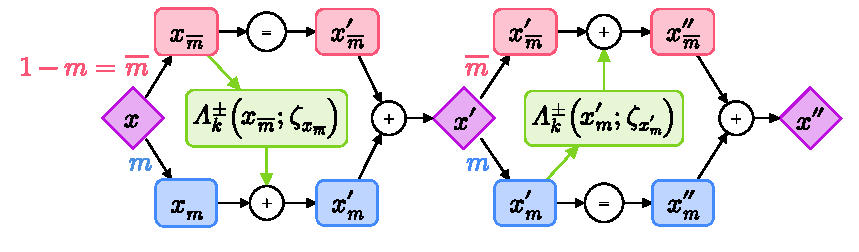
\includegraphics[width=\textwidth]{figures/splitx4.pdf}
   \caption{\label{fig:splitx}Illustration of the split \(x\) update.}
\end{figure}
%
As in HMC, we form a complete trajectory by performing \(N_{\mathrm{LF}}\) leapfrog steps in sequence, followed by a
Metropolis-Hastings accept/reject step as described in \Eqref{eq:mhcriteria}.
%
However, unlike in the expression for HMC, we must take into account the Jacobians of each of the transformations which
are easily computed to give
%
\begin{equation}
   \left|\tfrac{\partial v^{\prime}_{k}}{\partial v_{k}}\right| 
      = \exp{\left(\tfrac{\varepsilon}{2}s^{k}_{v}(\zeta_{v_{k}})\right)},\quad
   \left|\tfrac{\partial x^{\prime}_{k}}{\partial x_{k}}\right| 
      = \exp{\left(\varepsilon s^{k}_{x}(\zeta_{x_{k}})\right)}.
\end{equation}
%
In order to perform the updates in the generalized leapfrog integrator, we need to evaluate the functions
\(s, t, q\) in the respective updates.
%
We maintain separate networks with identical architectures for updating the \(x\) and \(v\) components separately.
%
For simplicity, we temporarily ignore the discrete leapfrog index \(k\), and restrict our attention to the \(s_{x},
t_{x}, q_{x}\) functions used in the \(x\) update equation, \(x_{k} = \Lambda^{+}(x;\zeta_{x})\) and note that the \(v\)
update (\Eqref{eq:new_momentum_update}) is identical.
%

Each of the \(s_{x}, t_{x}, q_{x}\) functions takes as input \(\zeta_{x} = (x, v, \tau)\), with \(x\in\mathbb{R}^{n}\),
\(v\in\mathbb{R}^{n}\), and \(\tau \in \mathbb{R}^{2}\).
%
The network splits these inputs and constructs the following intermediate variable
%
\begin{equation}
   z_{1} = \sigma(w_{x}^{T}x + w_{v}^{T}v + w_{\tau}^{T}\tau + b).
\end{equation}
%
This intermediate variable \(z_{1}\) is then passed through another series of fully-connected layers,
%
\begin{equation}
   z_{n} = \sigma(w_{n}^{T} z_{n-1} + b_{n}),\,\, z_{n-1}=\sigma(w_{n-2}^{T}z_{n-2} + b_{n-2}),\,\,%
   \ldots,\,\, z_{2} = \sigma(w_{2}^{T} z_{1} + b_{2}).
\end{equation}
%
The network outputs \(s_{x}, t_{x}, q_{x}\) are then defined in terms of this final hidden variable \(z_{n}\) as
%
\begin{equation}
   s_{x}(\zeta_{x}) = \alpha_{s}\tanh(w_{s}z_{n} + b_{s}),\quad
   t_{x}(\zeta_{x}) = w_{t}^{T}z_{n} + b_{t},\quad
   q_{x}(\zeta_{x}) = \alpha_{q}\tanh(w_{q}z_{n} + b_{q})
\end{equation}
%
where \(\alpha_{s}\), and \(\alpha_{q}\) are trainable scaling factors.
%
The only requirement on the details of the network is that the dimensionality of the outputs \(s_{x}, t_{x}, q_{x}\)
match the dimensionality of our physical variables \(x, v \in\mathbb{R}^{n}\).

%
%The network first passes each component through its own dense layer and then passes this sum through a subsequent series
%of layers to produce the desired output
%
% The network first splits the input and passes each component through a fully connected layer.
%
% These outputs are then summed together and passed through an activation function \(\sigma\) to construct the hidden
% variable
%
% these outputs through an activation function \(\sigma\),
% %
% \begin{equation}
%    z_{1} = \sigma(w_{x}^{T}x + w_{v}^{T}v + w_{\tau}^{T}\tau + b).
% \end{equation}
%
%

%
Next, we introduce a loss function
%
\begin{equation}
   \mathcal{L}_{\theta}{\left(\xi, \xi^{\prime}, A(\xi^{\prime}|\xi)\right)} = -\frac{\delta(\xi, \xi^{\prime})}{a^{2}}
\end{equation}
%
where \(\delta(\xi, \xi^{\prime})\) is a suitably chosen \emph{metric function}, and \(a\) is a scaling factor.


\subsubsection*{Acknowledgments}
This research used resources of the argonne leadership computing facility, which is a doe office of science user
facility supported under contract DE\_AC02--06CH11357.%
%
This work describes objective technical results and analysis.
%
Any subjective views or opinions that might be expressed in the work do not necessarily represent the views of the u.s.
doe or the united states government.

% Use unnumbered third level headings for the acknowledgments. All
% acknowledgments, including those to funding agencies, go at the end of the paper.


\bibliography{iclr2021_conference}
\bibliographystyle{iclr2021_conference}

\appendix
\section{Appendix}
\end{document}
